\subsection{Speed autopilot}\label{subsec:prob1.2}
We started studying the steady state characteristics of the surge speed as a function of propeller shaft velocity. 
\begin{figure}[H]
    \centering
    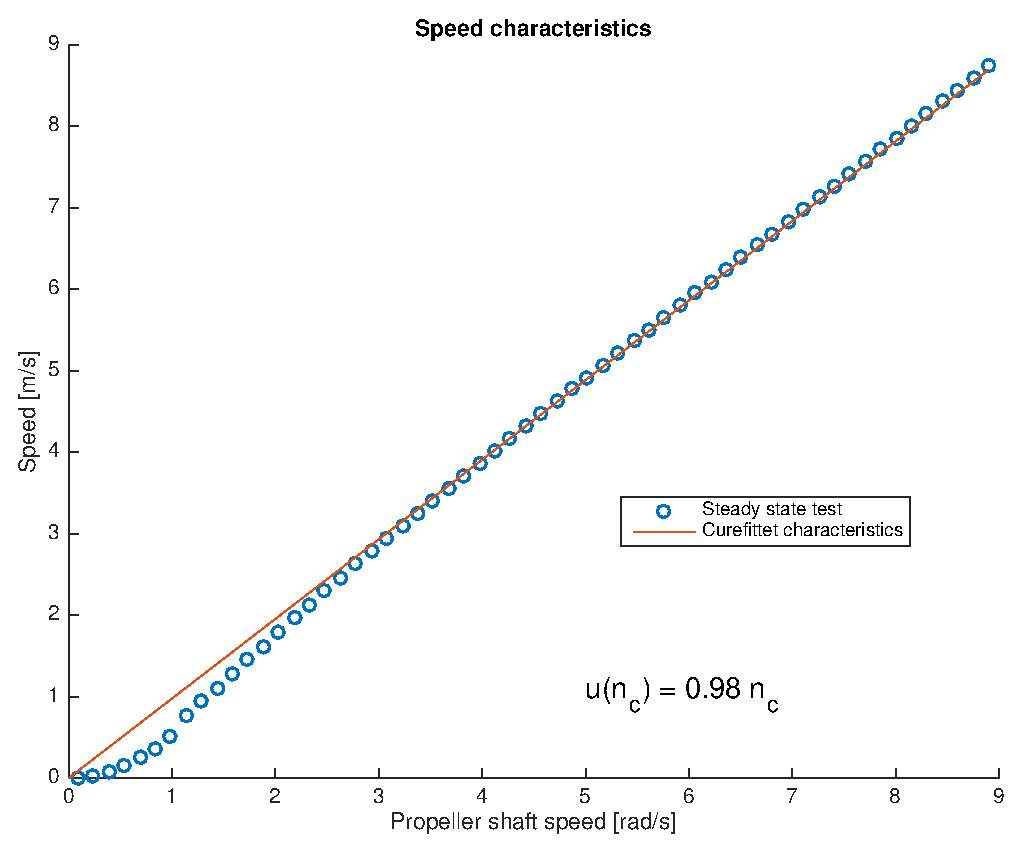
\includegraphics[width=0.8 \textwidth]{task1.8/Speed_characteristics}
    \caption{Speed characteristics}
    \label{fig:1.8-ss}
\end{figure}
As can be seen in figure \ref{fig:1.8-ss}, the characteristics of the ships surge speed is linear. This motivates a first or second order linear surge speed model, where the surge speed is decoupled from the rest of the system. We are assuming $$u>>v$$ which leads to: $$U=u$$ 
\subsubsection*{1.order linear model}
We then try a first order linear model.
\begin{equation}
\frac{u}{n_c}(s) = \frac{K}{1+Ts}
\end{equation}
Which gives us a quite good estimate of the speed dynamics (figure \ref{fig:1.8-speed-model}). Although we have a linear steady state relationship between shaft and surge speed, the time constant varies. This is a sign of a non-linear effect like quadratic damping.
\begin{figure}[H]
    \centering
    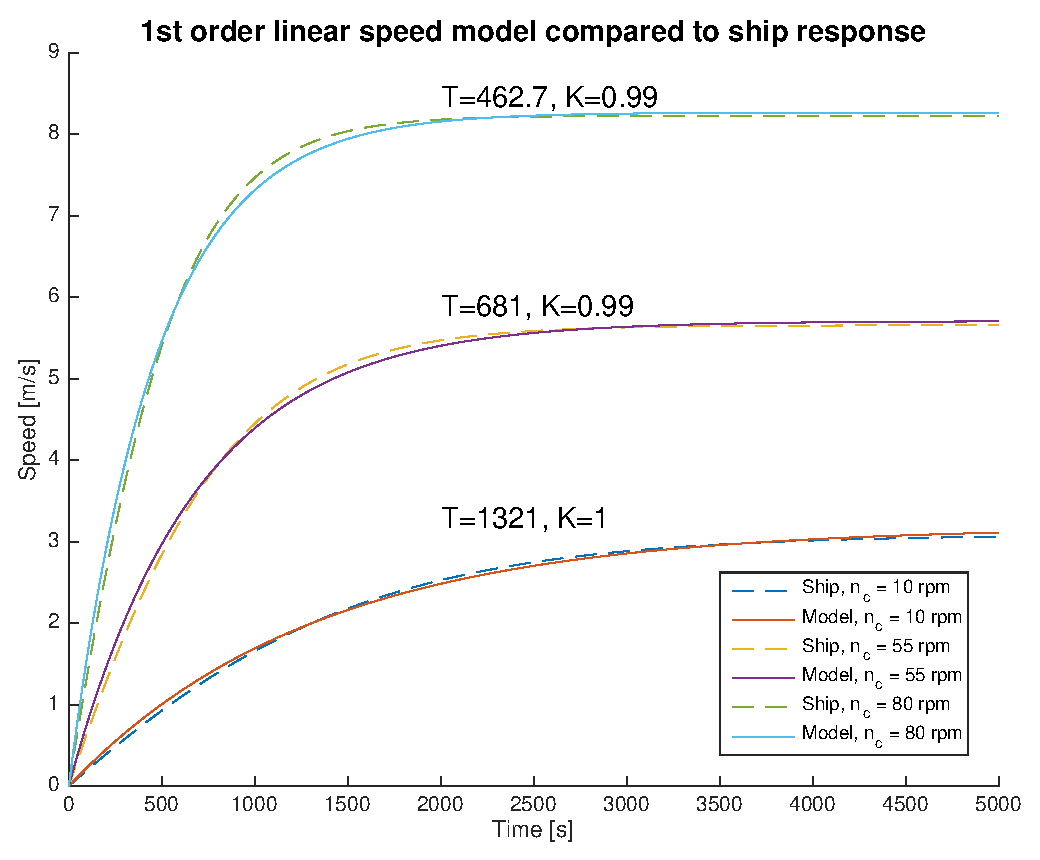
\includegraphics[width= \textwidth]{task1.8/Task1_8_speed_model}
    \caption{1.order linear speed model}
    \label{fig:1.8-speed-model}
\end{figure}
\subsubsection*{1.order quadratic model}
We also tried a quadratic model.
\begin{equation}
\dot{u} = \frac{n_c-K}{K_1 | u | u - K_2 u}
\end{equation}
Which gave a slightly better curve fit.
\begin{figure}[H]
    \centering
    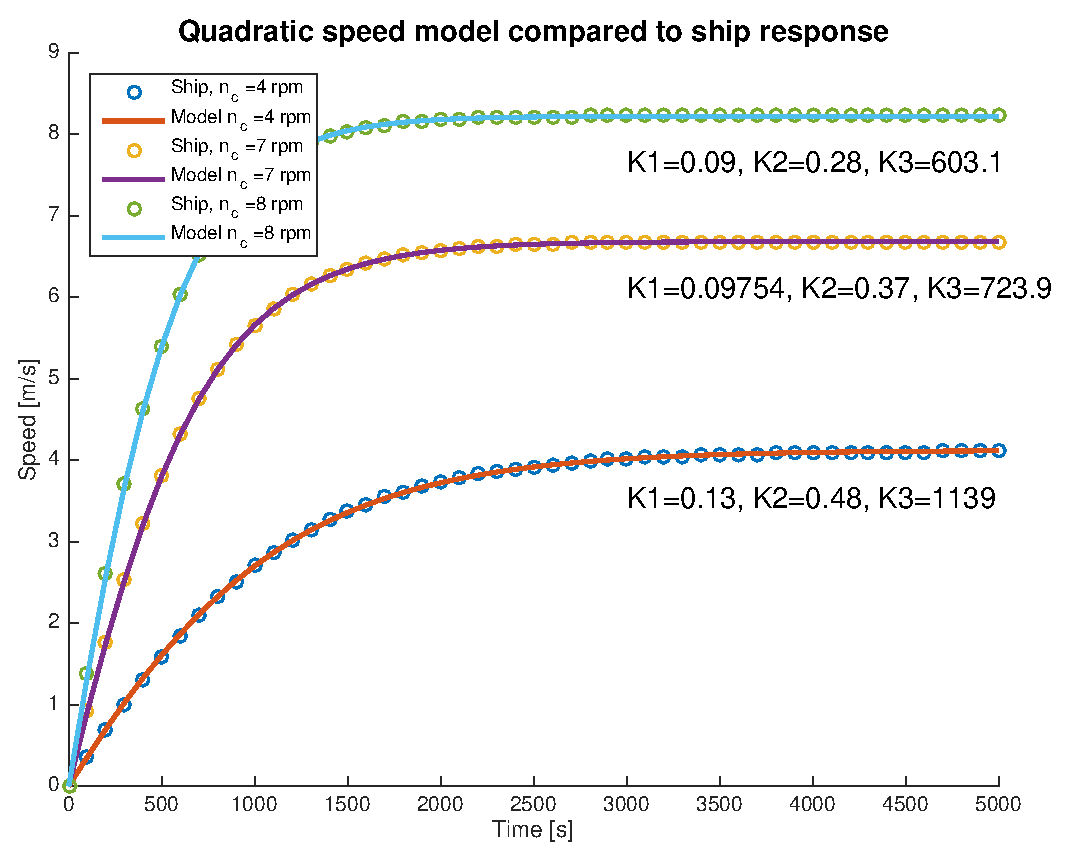
\includegraphics[width= 0.9\textwidth]{task1.8/Task1_8_quad_speed_model}
    \caption{1.order quadratic speed model}
    \label{fig:1.8-quad-speed-model}
\end{figure}
\subsubsection*{Speed model conclusion}
Both the linear and quadratic model where able to follow the ships response quite well. The quadratic is closer to reality, and will therefore be better when you need a more accurate model. For simpler analysis and controller, the linear model will do just fine. 

\subsubsection*{Controller}
The surge dynamics are stable and a PI controller will be able to reduce $\tilde{u}$ to zero. To improve the response of the controller, we added a force feed forward with the same gain as the steady state response. We then added a feedback PI-controller with anti-wind-up on the integral effect to take care of disturbances and modeling errors. The complete controller structure is shown in equation \ref{eq:speed-controller}. We also low pass filtered $u_d$ to avoid to fast changes in the speed reference. As in the heading controller, the LPF was set to slightly slower than the bandwidth of the surge dynamics. 
\begin{equation}
n_c = K_{ff} u_d - K_p \tilde{u} - K_i \int \tilde{u}
\label{eq:speed-controller}
\end{equation}

\subsubsection*{Step response}
The step response can be seen in figure \ref{fig:1.8-step}.
\begin{figure}[H]
    \centering
    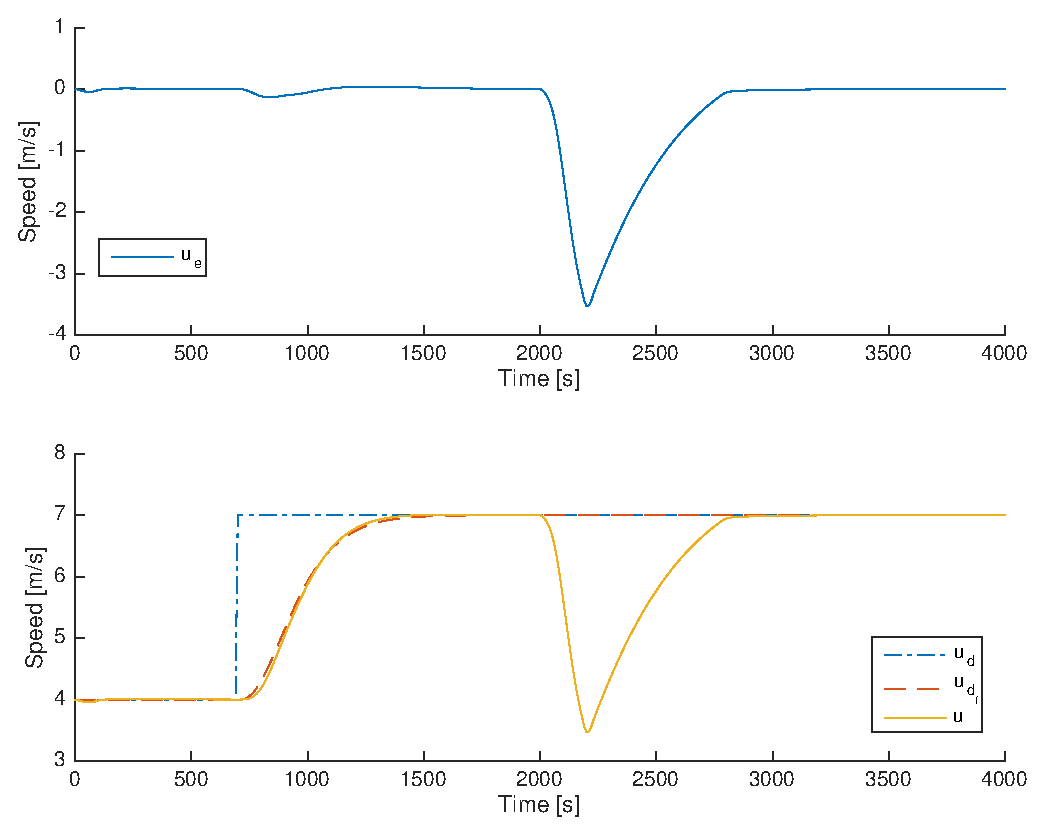
\includegraphics[width= \textwidth]{task1.8/Task1_8_sim}
    \caption{Speed step response}
    \label{fig:1.8-step}
\end{figure}